\chapter{The 2024 Paralympic Games in Paris}

\section{The City of Lights Welcomes the World}

\subsection{A Breathtaking Backdrop for Paralympic Excellence}
In 2024, the heart of France will beat to the rhythm of the Paralympic Games, as the iconic city of Paris welcomes athletes and spectators from across the globe. Renowned for its timeless beauty, rich history, and vibrant culture, Paris is set to provide a breathtaking backdrop for the extraordinary feats of Paralympic athletes. From the majestic Eiffel Tower to the historic Champs-Élysées, the city's landmarks will serve as inspiring symbols of human endeavor and resilience.

\subsection{Paris: A City Committed to Inclusivity}

Paris is not only a city of dreams but also a city committed to inclusivity. As it prepares to host the 2024 Paralympic Games, Paris has embarked on an ambitious journey to enhance accessibility and ensure a welcoming experience for all. The city's transformation includes adapting transportation systems, upgrading venues, and implementing innovative solutions to break down barriers and create a truly inclusive environment. From accessible public transport and accommodation to barrier-free access to stadiums and cultural sites, Paris is dedicated to providing a seamless and unforgettable experience for everyone involved in the Games.

\section{Schedule of Events}

\subsection{Twelve Thrilling Days of Paralympic Competition}

The Paris 2024 Paralympic Games will unfold over 12 thrilling days, showcasing a diverse array of sporting events that will captivate and inspire audiences worldwide. From the opening ceremony on August 28th to the closing ceremony on September 8th, Paris will be abuzz with the energy and excitement of Paralympic competition.

\begin{table}[h!]
\centering
\caption{2024 Paris Paralympic Schedule}
\begin{tabular}{l | c c c c c c c c c c c c}
\toprule
 & \multicolumn{8}{c}{\textbf{AUGUST}} & \multicolumn{4}{c}{\textbf{SEPTEMBER}} \\
 & 28 & 29 & 30 & 31 & 1 & 2 & 3 & 4 & 5 & 6 & 7 & 8 \\
\midrule
Ceremonies & \checkmark & & & & & & & & & & \checkmark \\
Blind Football & & \checkmark & \checkmark & \checkmark & \checkmark & \checkmark & \checkmark & & \checkmark & & & \\
Boccia & & & \checkmark & \checkmark & \checkmark & \checkmark & \checkmark & \checkmark & \checkmark & \checkmark & \checkmark & \checkmark \\
Goalball & & & \checkmark & \checkmark & \checkmark & \checkmark & \checkmark & \checkmark & \checkmark & \checkmark & \checkmark & \checkmark \\
Para Archery & & & \checkmark & \checkmark & \checkmark & \checkmark & \checkmark & \checkmark & \checkmark & \checkmark & \checkmark & \\
Para Athletics & & & & \checkmark & \checkmark & \checkmark & \checkmark & \checkmark & \checkmark & \checkmark & \checkmark & \checkmark \\
Para Badminton & & & & \checkmark & \checkmark & \checkmark & \checkmark & \checkmark & \checkmark & \checkmark & \checkmark & \checkmark \\
Para Canoe & & & & & & & & & \checkmark & \checkmark & \checkmark & \checkmark \\
Para Cycling Road & & & & \checkmark & \checkmark & \checkmark & & & & & & \\
Para Cycling Track & & & & & \checkmark & \checkmark & \checkmark & \checkmark & \checkmark & \checkmark & & \\
Para Equestrian & & & & & & \checkmark & \checkmark & \checkmark & & & & \\
Para Judo & & & & & & & \checkmark & \checkmark & \checkmark & \checkmark & & \\
Para Powerlifting & & & & & & & \checkmark & \checkmark & \checkmark & \checkmark & \checkmark & \\
Para Rowing & & \checkmark & \checkmark & \checkmark & \checkmark & \checkmark & \checkmark & \checkmark & & & & \\
Para Swimming & & & & \checkmark & \checkmark & \checkmark & \checkmark & \checkmark & \checkmark & \checkmark & \checkmark & \checkmark \\
Para Table Tennis & & & \checkmark & \checkmark & \checkmark & \checkmark & \checkmark & \checkmark & \checkmark & \checkmark & \checkmark & \checkmark \\
Para Taekwondo & & & & & & & & \checkmark & \checkmark & \checkmark & \checkmark & \\
Para Triathlon & & & & & & & & & & \checkmark & & \\
Shooting Para Sport & & & & \checkmark & \checkmark & \checkmark & \checkmark & \checkmark & \checkmark & \checkmark & & \\
Sitting Volleyball & & & \checkmark & \checkmark & \checkmark & \checkmark & \checkmark & \checkmark & \checkmark & \checkmark & \checkmark & \\
Wheelchair Basketball & & & & & \checkmark & \checkmark & \checkmark & \checkmark & \checkmark & \checkmark & \checkmark & \\
Wheelchair Fencing & & & & \checkmark & \checkmark & \checkmark & \checkmark & \checkmark & \checkmark & \checkmark & & \\
Wheelchair Rugby & & & & & & \checkmark & \checkmark & \checkmark & \checkmark & \checkmark & & \\
Wheelchair Tennis & & & \checkmark & \checkmark & \checkmark & \checkmark & \checkmark & \checkmark & \checkmark & \checkmark & \checkmark & \checkmark \\
\bottomrule
\end{tabular}
\end{table}

\subsection{Witnessing Athleticism and Determination}

Spectators will have the opportunity to witness a wide range of Paralympic sports, from the iconic track and field events at the Stade de France to the thrilling wheelchair basketball matches at the Accor Arena.  Each day will bring new opportunities to witness the extraordinary athleticism and determination of Paralympic athletes as they push their limits and strive for greatness.

\section{Athletes to Watch}

\subsection{Stories of Triumph and Resilience}

The Paris 2024 Paralympic Games will feature a constellation of talented athletes, each with their own unique story of triumph and resilience. These athletes have overcome challenges, defied expectations, and emerged as beacons of inspiration for people around the world. Their stories of perseverance, dedication, and unwavering belief in their abilities will undoubtedly capture the hearts of spectators and leave a lasting legacy.

\begin{figure}[h!]
    \centering
    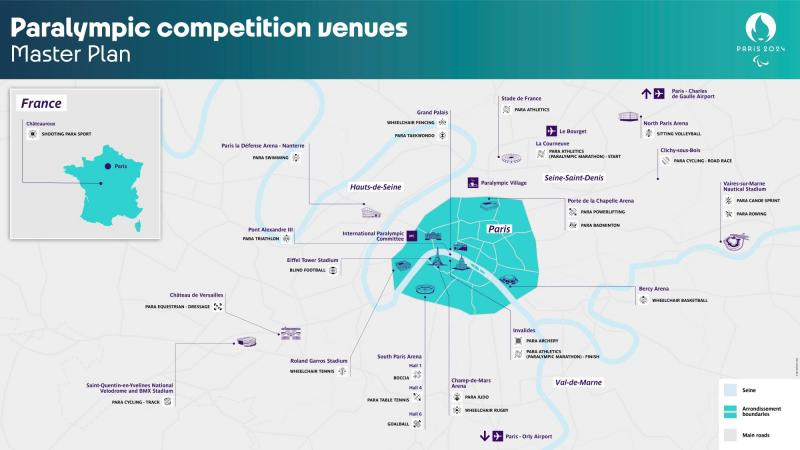
\includegraphics[width=\textwidth]{Images/Venues.jpg} % Replace with the actual filename of your map image
    \caption{Map of Paralympic Venues in Paris (Source: PARIS 2024 Comité d'Organisation des Jeux Olympiques et Paralympiques (COJOP))}
    \label{fig:venues_map}
\end{figure}

\subsection{Paralympic Stars to Shine in Paris}


\begin{enumerate}
\item Beatrice Vio (Italy) - Wheelchair Fencing
    \begin{itemize}
    \item \textbf{Background and Achievements:} Beatrice Vio, affectionately known as "Bebe," is a force to be reckoned with in the world of wheelchair fencing. At just 25 years old, she has already amassed an impressive collection of accolades, including multiple Paralympic and World Championship gold medals. Her lightning-fast reflexes, tactical brilliance, and unwavering determination have made her a dominant figure in the sport.
    \item \textbf{Personal Story:} Bebe's journey to Paralympic glory is nothing short of inspirational. At the age of 11, she contracted meningitis, which led to the amputation of all four limbs. Despite facing immense challenges, she refused to let her disability define her. With the support of her family and a passion for fencing, she adapted to her new reality and quickly rose through the ranks of wheelchair fencing, becoming a role model for aspiring athletes worldwide.
    \item \textbf{Goals and Aspirations:} Bebe's sights are firmly set on defending her Paralympic title in Paris 2024. She is driven by a desire to continue pushing the boundaries of her sport and inspire others to embrace their own potential, regardless of their circumstances. Her infectious enthusiasm and unwavering spirit make her a true ambassador for the Paralympic movement.
    \end{itemize}

\item Markus Rehm (Germany) - Para Athletics (Long Jump)
    \begin{itemize}
    \item \textbf{Background and Achievements:} Markus Rehm, known as "Blade Jumper," is a Paralympic long jump legend. He has shattered records and redefined the possibilities of his sport with his incredible leaping ability. Rehm is a multiple Paralympic and World Champion, and his personal best jump of 8.62 meters is farther than the winning jump in the 2020 Tokyo Olympics. 
    \item \textbf{Personal Story:} Rehm lost his right leg in a wakeboarding accident at the age of 14. Undeterred, he turned to athletics and discovered his talent for long jump. With the aid of a carbon fiber prosthetic blade, he has soared to extraordinary heights, consistently outperforming many able-bodied athletes. Rehm's story is a testament to the power of resilience, determination, and the ability to turn adversity into triumph.
    \item \textbf{Goals and Aspirations:} In Paris 2024, Rehm aims to continue his dominance in the long jump and further solidify his legacy as one of the greatest Paralympic athletes of all time. He also hopes to use his platform to advocate for greater inclusion and opportunities for people with disabilities in sports and beyond.
    \end{itemize}
\end{enumerate}

\section{Beyond the Competition: Cultural and Social Impact}

\subsection{Challenging Stereotypes, Promoting Inclusion}
The Paralympic Games transcend the realm of sports, acting as a powerful catalyst for cultural and social change. They challenge deeply ingrained stereotypes about disability, showcasing the extraordinary abilities and achievements of Paralympic athletes and inspiring a shift in societal perceptions. By promoting inclusivity, accessibility, and equality, the Games encourage a more accepting and understanding world where everyone, regardless of their abilities, can fully participate and contribute.

\subsection{A Lasting Legacy for Paris and Beyond}

The legacy of the Paris 2024 Paralympic Games is expected to extend far beyond the closing ceremony. The city's commitment to accessibility and inclusion will leave a lasting impact, creating a more welcoming and barrier-free environment for people with disabilities. The Games will also serve as a powerful educational tool, raising awareness and understanding of disability among the general public. By showcasing the resilience, determination, and triumphs of Paralympic athletes, Paris 2024 has the potential to inspire future generations and foster a more inclusive society where everyone can thrive.
